\documentclass[border=10pt]{standalone}
\usepackage{tikz}
\usepackage{amsmath,amssymb}

\usetikzlibrary{arrows.meta, positioning, fit, backgrounds}

\begin{document}
% if plate p binds index i and variable v appears in p, then v should vary over
% i
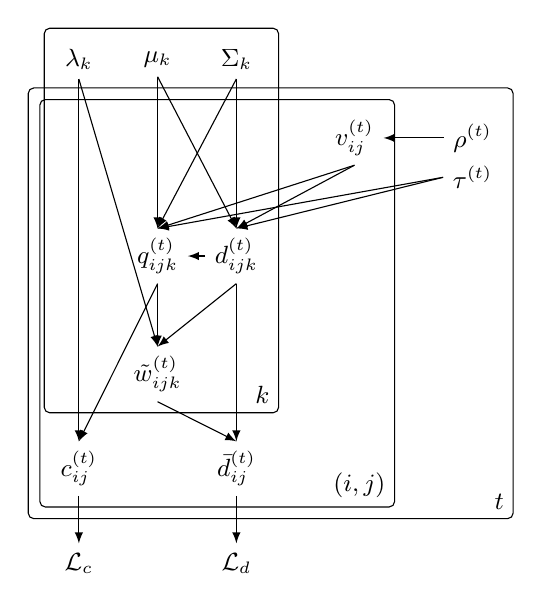
\begin{tikzpicture}[
    node distance=1cm and 1cm,
    >={Stealth[length=2mm]},
    every node/.style={font=\small},
    every edge/.style = {draw, -latex}
]

% Define coordinates for nodes
\node (lambdak) at ( -1, 5) {$\lambda_k$};
\node (muk)  at (  0, 5) {$\mu_k$};
\node (Sigmak)     at (  1, 5) {$\Sigma_k$};

\node (vij)     at (2.5, 4) {$v_{ij}^{(t)}$};
\node (rho)     at (  4, 4) {$\rho^{(t)}$};

\node (tau)     at (  4, 3.5) {$\tau^{(t)}$};

\node (qijk)    at (  0, 2.5) {$q_{ijk}^{(t)}$};
\node (dijk)    at (  1, 2.5) {$d_{ijk}^{(t)}$};

\node (wijk)    at (  0, 1) {$\tilde{w}_{ijk}^{(t)}$};

\node (cij)     at ( -1, -0.2) {$c_{ij}^{(t)}$};
\node (dijbar)  at (  1, -0.2) {$\bar{d}_{ij}^{(t)}$};

\node (Lc)      at ( -1, -1.4) {$\mathcal{L}_c$};
\node (Ld)      at (  1, -1.4) {$\mathcal{L}_d$};


\draw (Sigmak.south) edge (qijk.north) edge (dijk.north)
      (muk.south) edge (qijk.north) edge (dijk.north)
      (vij.south) edge (qijk.north) edge (dijk.north)
      (rho.west) edge (vij.east)
      (tau.west) edge (qijk.north) edge (dijk.north)
      (lambdak.south) edge (wijk.north) edge (cij.north)
      (qijk.south) edge (wijk.north) edge (cij.north)
      (dijk.south) edge (wijk.north) edge (dijbar.north)
      (dijk.west) edge (qijk.east)
      (wijk.south) edge (dijbar.north)
      (cij) edge (Lc)
      (dijbar) edge (Ld);

% Inner plate k
\begin{scope}[on background layer]
    \node[draw, rectangle, rounded corners=2pt, 
          inner sep=4pt,
          fit=(Sigmak)(muk)(lambdak)(wijk)(dijk),
          label={[anchor=south east, font=\small]south east:$k$}] (plate_k) {};
\end{scope}

% Middle plate (i,j)
\begin{scope}[on background layer]
    \node[draw, rectangle, rounded corners=2pt,
          inner sep=4pt,
          fit=(wijk)(dijk)(vij)(cij)(dijbar),
          label={[anchor=south east, font=\small]south east:$(i,j)$}] (plate_ij) {};
\end{scope}

% Outer plate t
\begin{scope}[on background layer]
    \node[draw, rectangle, rounded corners=2pt,
          inner sep=4pt,
          fit=(plate_ij)(rho)(tau),
          label={[anchor=south east, font=\small]south east:$t$}] (plate_t) {};
\end{scope}

\end{tikzpicture}
\end{document}
